\chapter{Conclusão}

Este trabalho apresentou o processo de implementação do \textit{walking gait} do time AUTUofM, descrevendo as soluções de software e justificando as decisões tomadas. Apresentou-se a abordagem tomada para mover a implementação da placa microcontroladora \textit{OpenCM9.04} para um \textit{software} dentro do controlador principal.

Para tanto, foram realizadas modificações no \textit{firmware} da \textit{OpenCM9.04} criando um componente \textit{Proxy} que encaminha os comandos recebidos através da porta \textit{USB} aos motores. Comandos estes gerados pela nova implementação do \textit{walking gait}, desta vez utilizando a linguagem C++. O mesmo método usando um padrão de trajetórias senoidais e recuperação de distúrbios proposto por Karimi \textit{et al} foi utilizado para a nova implementação.

\begin{figure}[htb]
	\centering
	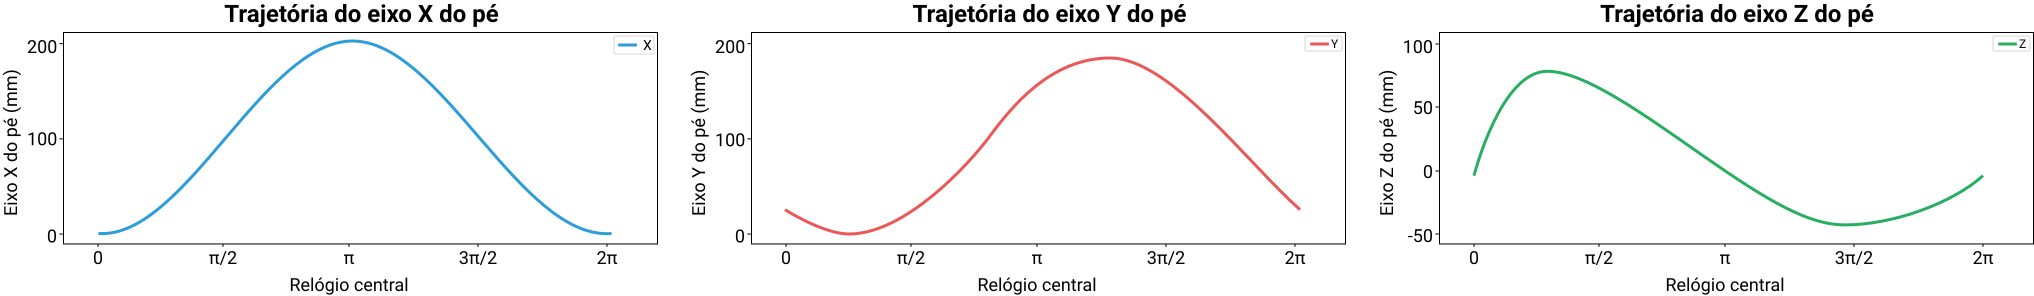
\includegraphics[width=\textwidth]{imagens/svg/conclusion-trajectories-graph}
	\caption{Gráficos das trajetórias do ciclo de caminhada nos eixos X, Y e Z gerados pela nova implementação do \textit{walking gait}.}
	\label{fig:conclusion:trajectories:graph}
\end{figure}

\begin{figure}[htb]
	\centering
	\includegraphics[width=\textwidth]{imagens/conclusion-trajectories-graph-old}
	\caption{Gráficos das trajetórias do ciclo de caminhada nos eixos X, Y e Z gerados Karimi \textit{et al}.}
	\label{fig:conclusion:trajectories:graph:old}
\end{figure}

Devido a falta de dados concretos sobre a geração das trajetórias, foram utilizadas comparações visuais com os gráficos fornecidos por Karimi \textit{et al} em seu trabalho. Nas figuras \ref{fig:conclusion:trajectories:graph} e \ref{fig:conclusion:trajectories:graph:old} é possível observar, respectivamente, os gráficos das trajetórias geradas pelo novo e pelo velho \textit{walking gait}. Em ambas as imagens possível observar a trajetória nos eixos $X$, $Y$ e $Z$ separados. No eixo vertical do gráfico o trajetória é escalada em milímetros. No eixo horizontal a escala é no ciclo do relógio central.

Ainda na figura~\ref{fig:conclusion:trajectories:graph:old} observa-se uma linha vermelha pontilhada, que indica a compensação realizada pelo sistema durante um evento de distúrbio realizado no robô físico \cite{karimionline}. Tal evento não foi possível de ser reproduzido pela falta de acesso ao robô físico.

Em relação ao movimento da caminhada, foi possível validar a geração da cinemática inversa através das animações, em tempo real, produzidas pelo visualizador 3D. A figura~\ref{fig:conclusion:arash:frames} observa-se 4 \textit{capturas de tela} do visualizador em uma caminhada com $V_x = 0.5$ da perspectiva lateral, na primeira linha, e pela perspectiva frontal na segunda linha. Nas primeira coluna, $t = 0$, observa-se o mostra uma posição estável, com ambos os pés no chão. Na segunda, observa-se o momento em que o pé direito é levantado, onde $t = \pi/2$. A terceira coluna mostra o momento em que $t = \pi$, metade do ciclo, em que ambos os pés voltam a tocar no chão. Então, a quarta coluna mostra o momento em que o pé esquerdo sai do chão, $t = 3\pi/2$. Seguindo o ciclo, o relógio é reiniciado e o estado retorna ao da primeira coluna.

\begin{figure}[htb]
	\centering
	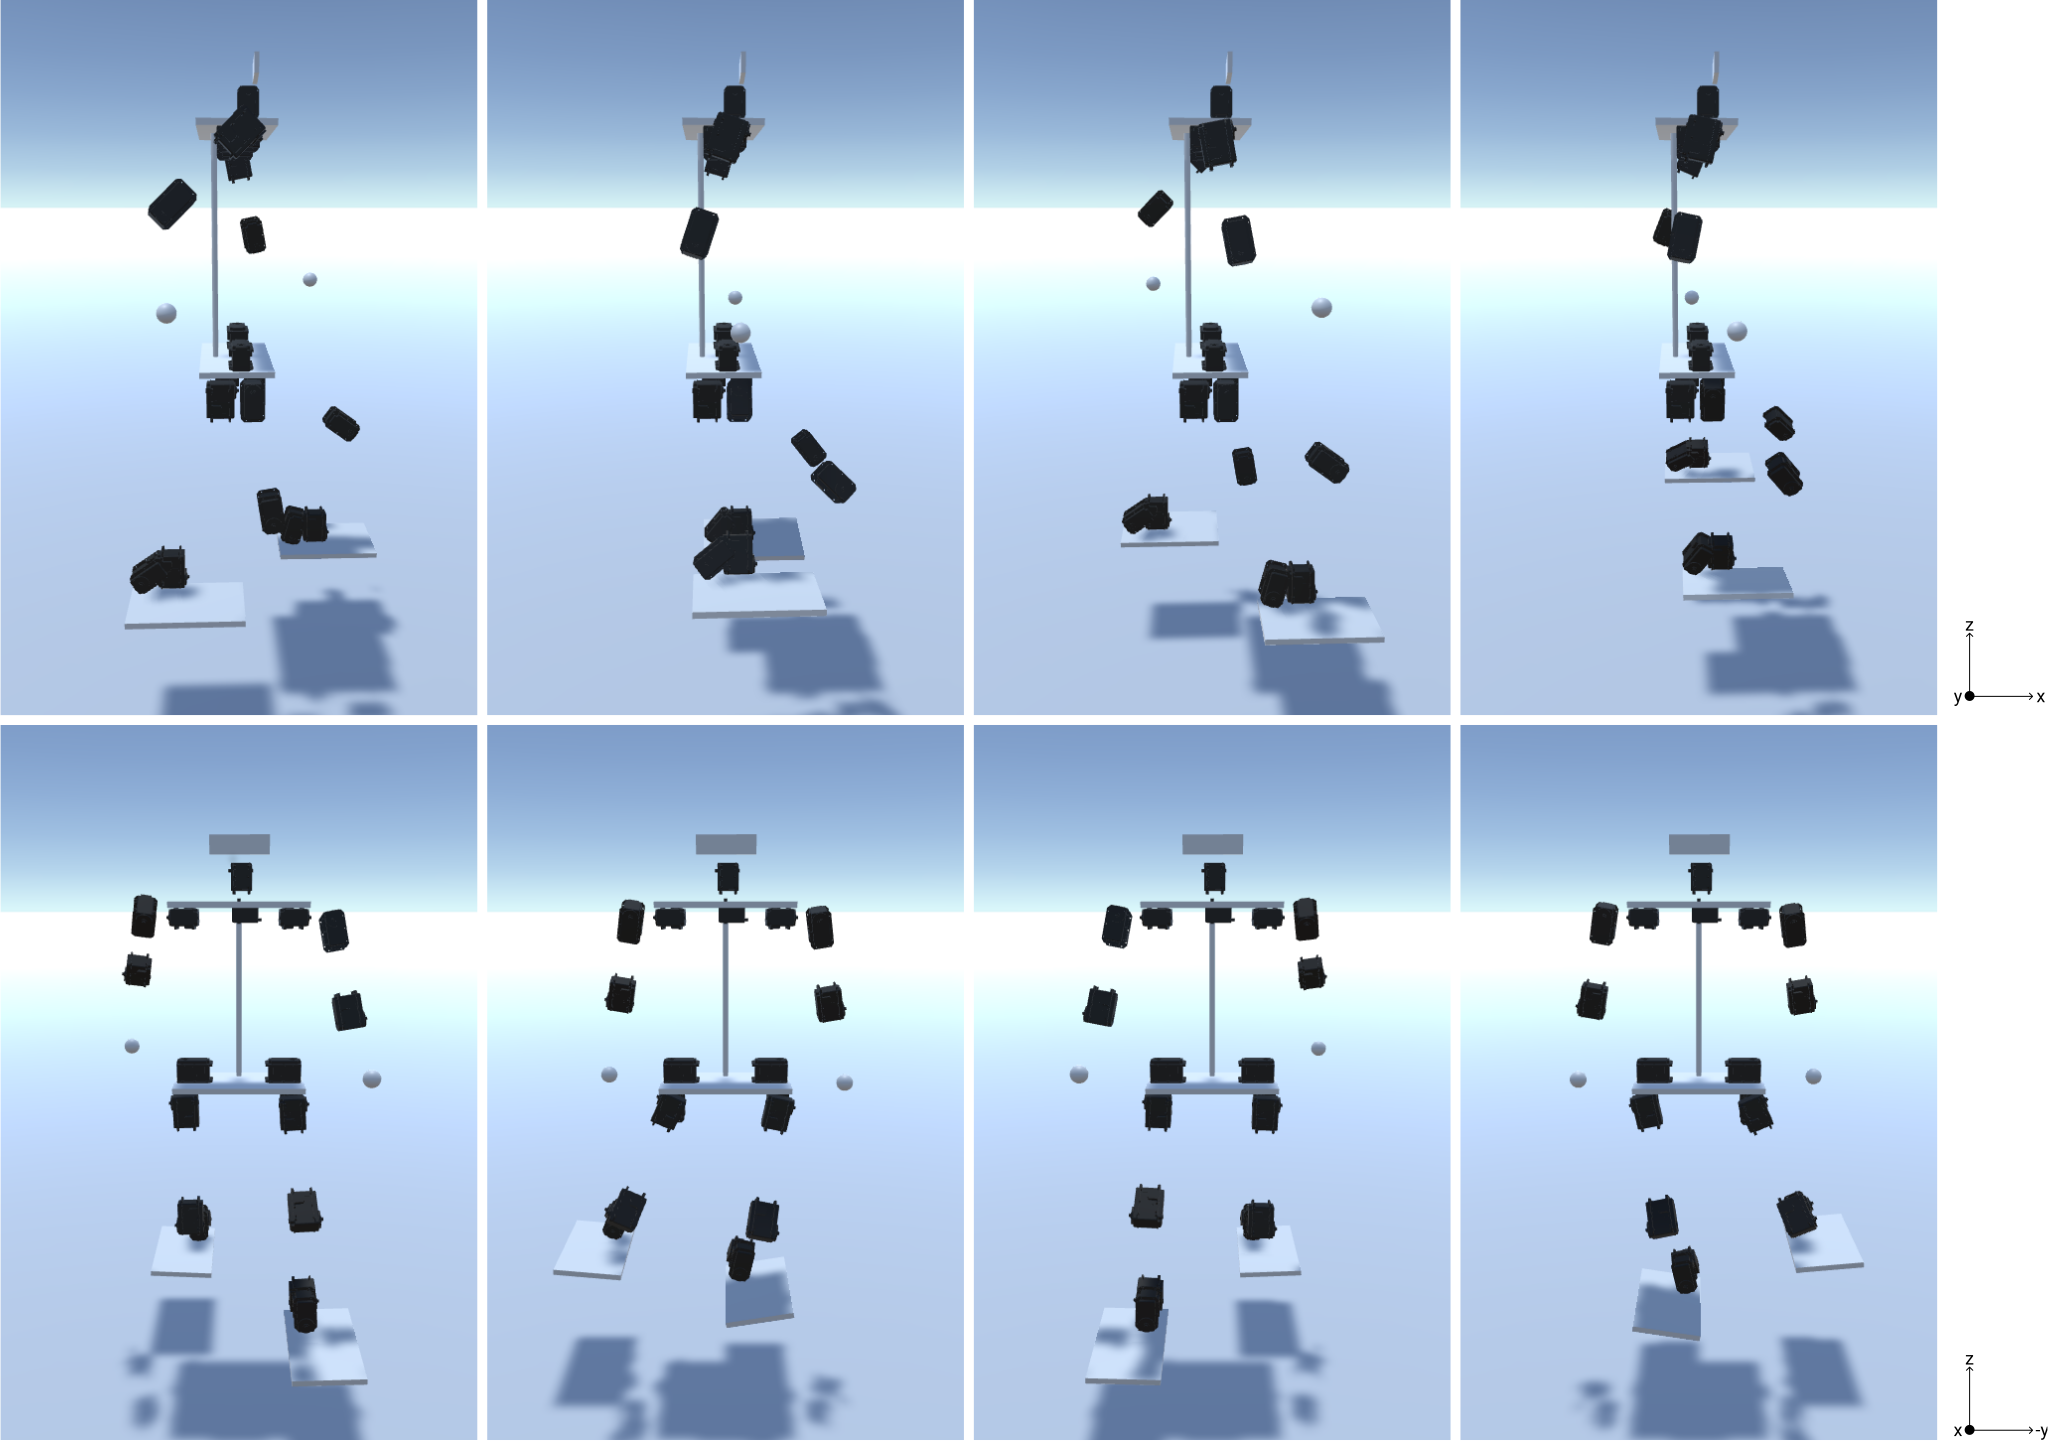
\includegraphics[width=\textwidth]{imagens/svg/conclusion-arash-frames}
	\caption{Visualização frontal e lateral dos movimentos da caminhada.}
	\label{fig:conclusion:arash:frames}
\end{figure}

Um esquema de configurações persistidas em disco em arquivos JSON atacou diretamente o problema da falta de controle sobre as configurações geradas. Assim, os arquivos de configuração podem ser versionados utilizando algum sistema de versionamento de código.

Apesar da simulação não ter sido implementada neste trabalho, seu futuro acomplamento será menos complexo, já que a nova implementação usa o conceito de um sistema distribuído baseado em serviços.

Considerando que o \textit{walking gait} funciona dentro do controlador principal. Futuras melhorias que possam exigir mais recursos -- processamento ou memórias RAM e ROM -- podem ser implementadas.

Finalmente, de acordo com os resultados obtidos, podemos concluir que a implementação do \textit{walking gait} foi realizada e pode ser utilizada como base para diversas melhorias descritas na seção~\ref{sec:conclusion:future}.

\section{Trabalhos futuros}
\label{sec:conclusion:future}

As atualizações realizadas no \textit{walking gait} original do time AUTUofM agora permitem diversas expensões no código para futuras atualizações e investigações. Assim, os próximos parágrafos descrevem alguns possíveis trabalhos futuros.

Este trabalho foi todo desenvolvido apenas usando \textit{software} e visualização 3D dos ângulos gerados. A implementação e teste usando o robô real é um passo fundamental para a consolidação deste trabalho.

A implementação sem a utilização de um sistema de simulação apropriado não garante que o robô realmente possa caminhar. O uso do visualizador 3D apenas mostra um esboço do movimento, sem a real caminhada. Em paralelo, embora os dados do leitor de orientação sejam levados em conta tem todos os cálculos, seus efeitos não foram testados. Consequentemente, a integração do módulo do \textit{walking gait} a um \textit{framework} de simulação é um passo em direção a um sistema mais completo.

Segundo, durante uma tarefa genérica realizada por um robô não apenas se caminha. Movimentos como chutes, levantar-se do chão, pegar um copo -- entre outros -- são normalmente pré-gravados na etapa de desenvolvimento e durante a tarefa são apenas reproduzidos. Desta forma, um módulo para gravar e reproduzir estes movimentos faz-se necessário.

Terceiro, o fato do \textit{walking gait} rodar fora da \textit{OpenCM9.04} adiciona algum atraso extra entre o cálculo dos ângulos e a aplicação aos motores. Adicionalmente, os dados processados do leitor de orientação demoram mais a ter efeito nos cálculos das correções. Porém, o seu impacto real, durante a caminhada, não pode ser explorado neste trabalho deixando esta investigação para trabalhos futuros.

Quarto, alguns métodos de caminhada utilizam sensores nos pés de forma a detectar quando há o contato com o chão. Este momento é crítico pois, em caso de algum distúrbio, se houver uma diferença do momento esperado para o momento real do toque, ações diferenciadas poderão ser tomadas. Com isto em mente, sabe-se que os motores da série \textit{MX} possuem \textit{feedback} de carga baseado na voltagem de saída interna, onde deverá ser possível medir a diferença nas cargas esperadas e reais afim de prever se o pé está em contato com o chão.

Finalmente, outros métodos mais complexos de caminhada, utilizando mais processamento e mais memória, poderão ser implementados já que a barreira de recursos do \textit{OpenCM9.04} foi quebrada.